\section{Gestión de Personal}
\subsection{Autoevaluación}
En esta sección se han cumplido los objetivos correspondientes al 10.
\subsection{Introducción}
\paragraph{}
En cuanto a la gestión de recursos humanos Odoo ofrece un conjunto de módulos que incluyen herramientas para su realización. En ella se engloba los procesos de reclutamiento y de la gestión del personal una vez que han sido contratados. De esta manera permite a las organizaciones gestionar eficientemente el reclutamiento para cada etapa del proceso, definir criterios de evaluación y mantener un registro de los postulantes. Por otro lado, gestiona la información de los empleados, evaluar su desempeño y asignar responsabilidades.
\subsection{Metodología}
\paragraph{}
Para comprobar el funcionamiento de este aspecto en Odoo se ha instalado los módulos de \textit{Proceso de selección} y \textit{Empleados}. En el módulo de Empleados se han creado varios departamentos desde el menú de departamentos, en la empresa raíz CochesMA se ha creado un departamento de Administración, Ventas y Servicios profesionales, en la rama de CochesMA.UK se ha creado un departamento de Gestión y otro de Ventas y en la rama de CochesMA.US se ha creado uno uno de Personal y otro de Servicios profesionales. Para cada uno durante la creación del mismo se ha asignado un gerente de entre las personas que se han creado en la sección de configuración funcional.
\paragraph{}
Además, dentro del menú configuración del módulo \textit{Empleados} se puede acceder al menú \textit{Puestos de trabajo}. Desde aquí se pueden crear puestos de trabajo rellenando la información necesaria en el formulario de creación, en este caso se ha creado dos director técnico, dos responsables de comunicación y ventas, dos gestores de personal, dos directores ejecutivos  y un consultor asignando cada uno a la empresa raíz o a una de las ramas. 
\paragraph{}
En cuanto al proceso de reclutamiento, vamos a simular una operación en el que se va a contratar a una persona para el departamento de \textit{Ventas} con al menos un año de experiencia en operaciones internacionales con suiza y que sepa Francés y Alemán. Para ello, se ha creado un nuevo puesto de trabajo Director de marketing como se ha explicado anteriormente y se añadido una descripción explicando en que consiste el puesto y los requisitos para ello. Además, desde el menú de Tipo de habilidad en el módulo de Reclutamiento se ha creado una entrada llamada \textit{Languages}, en el que se valoran idiomas como el Alemán, Francés, Inglés y Español, con niveles desde bajo, medio y avanzado. Por otro lado, también se ha creado un nuevo tipo de habilidad llamada experiencia la cual tiene como posibilidad operaciones internacionales con suiza, con distintos niveles según el tiempo de experiencia, 1, 2 o 3 años. También, se ha ido a configuración del módulo de Reclutamiento y se ha activado la opción de Pantalla de CV. Además, se ha definido un formulario de entrevista que tendrá que rellenar el candidato, para ello se ha hecho clic en los 3 puntos del puesto de trabajo en el módulo de reclutamiento y seleccionar la opción de Nuevo Formulario de entrevista y a continuación se ha rellenado con las siguientes 3 preguntas. Para que Odoo permita enviar el formulario creado se ha activado la opción de Enviar encuesta de entrevista en los ajustes del módulo.
\begin{figure}[h]
    \centering
    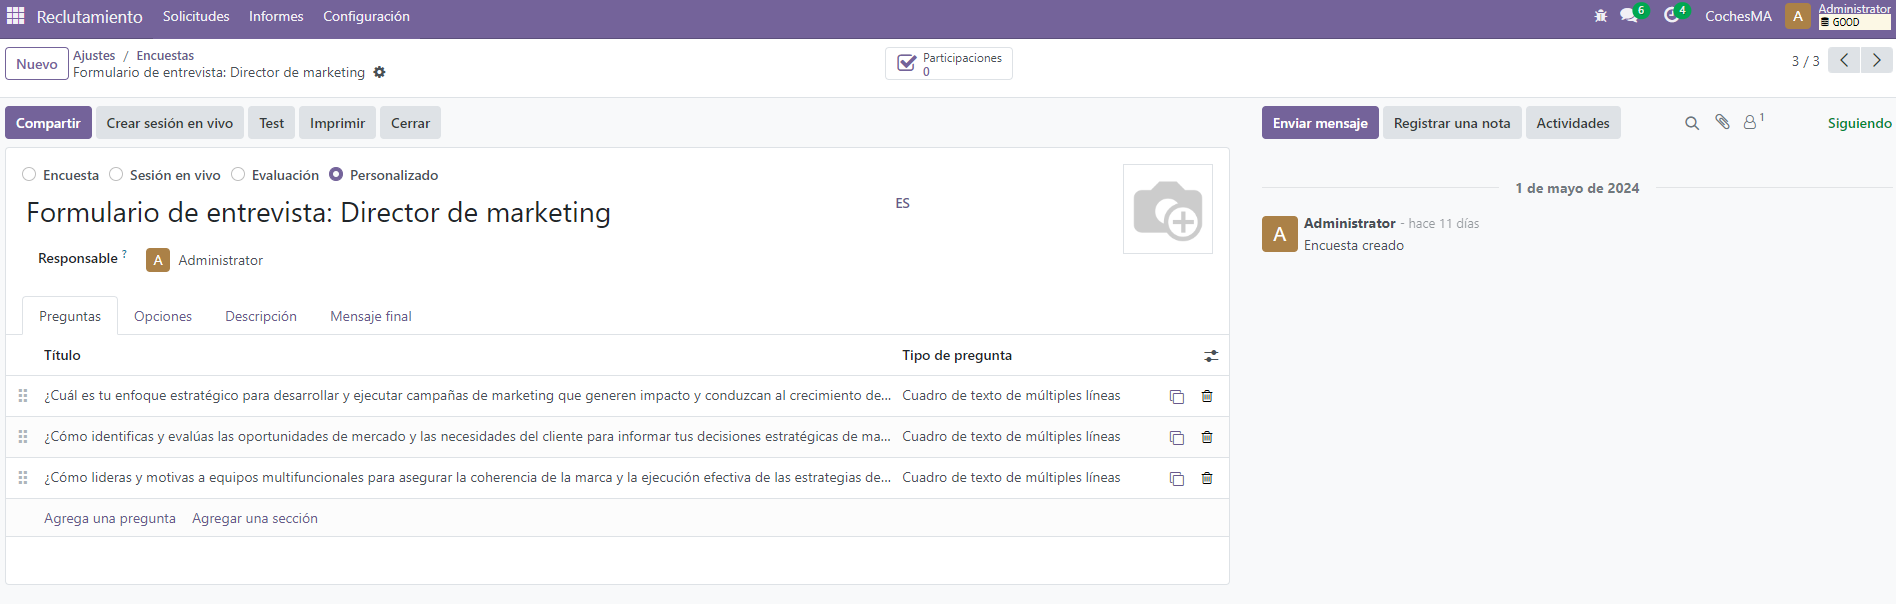
\includegraphics[width=1\linewidth]{fotosGestPers/image.png}
    \caption{Formulario de entrevista para el puesto de Director de marketing}
    \label{fig:enter-label}
\end{figure}
\paragraph{}
A continuación, en el modulo de reclutamiento se ha hecho clic al enlace Página de trabajos del puesto de Director de marketing. Se ha rellenado el formulario de la solicitud con la información correspondiente y se ha añadido el currículum y se ha enviado. Desde el módulo de Reclutamiento se ha podido ver la solicitud del puesto. Se ha hecho clic en él y se ha asignado en la opción de habilidades un nivel avanzado de Alemán y Francés y 1 año de experiencia en operaciones internacionales con suiza. Se ha realizado el proceso de reclutamiento con dos entrevistas se ha propuesto un contrato y se ha firmado. Finalmente, se ha creado un usuario de tipo empleado para el nuevo Director de marketing.
\subsection{Resultados y análisis}
\paragraph{}
Durante este apartado se ha creado en la compañía matriz un departamento de Administración, de Ventas y de Servicios profesionales, en la rama CochesMA.UK un departamento de Gestión y de Ventas y en la rama CochesMA.US un departamento de Personal y de Servicios profesionales. 
\begin{figure}[h]
    \centering
    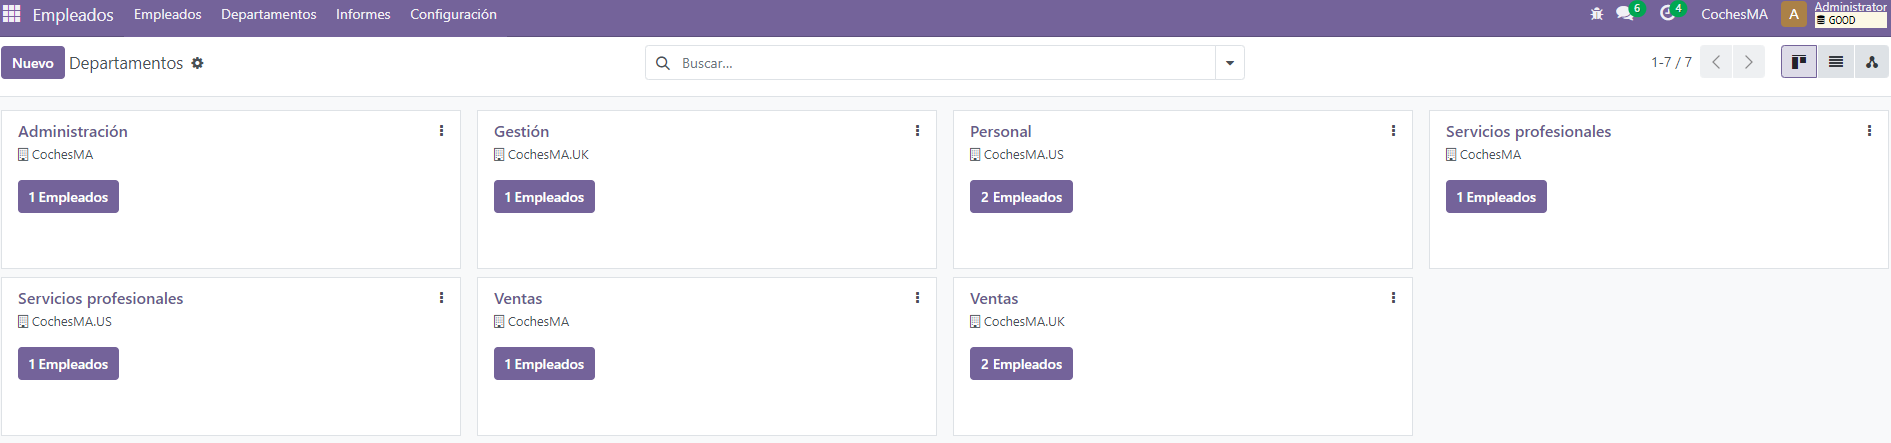
\includegraphics[width=1\linewidth]{fotosGestPers/departamentos.png}
    \caption{Lista de departamentos de la compañía}
    \label{fig:enter-label}
\end{figure}
\paragraph{}
Además, se han creado los siguientes puestos de trabajo dentro de cada departamento. Para el departamento de Administración un puesto de Director Ejecutivo, para el de Servicios profesionales un Director Técnico y un consultor, para el de Personal un Gestor de personal y para el Ventas un Responsable de comunicación y ventas. Se han creado 9 empleados, tantos como usuarios había y se han distribuido entre los puestos de trabajo. 
\begin{figure}[h]
    \centering
    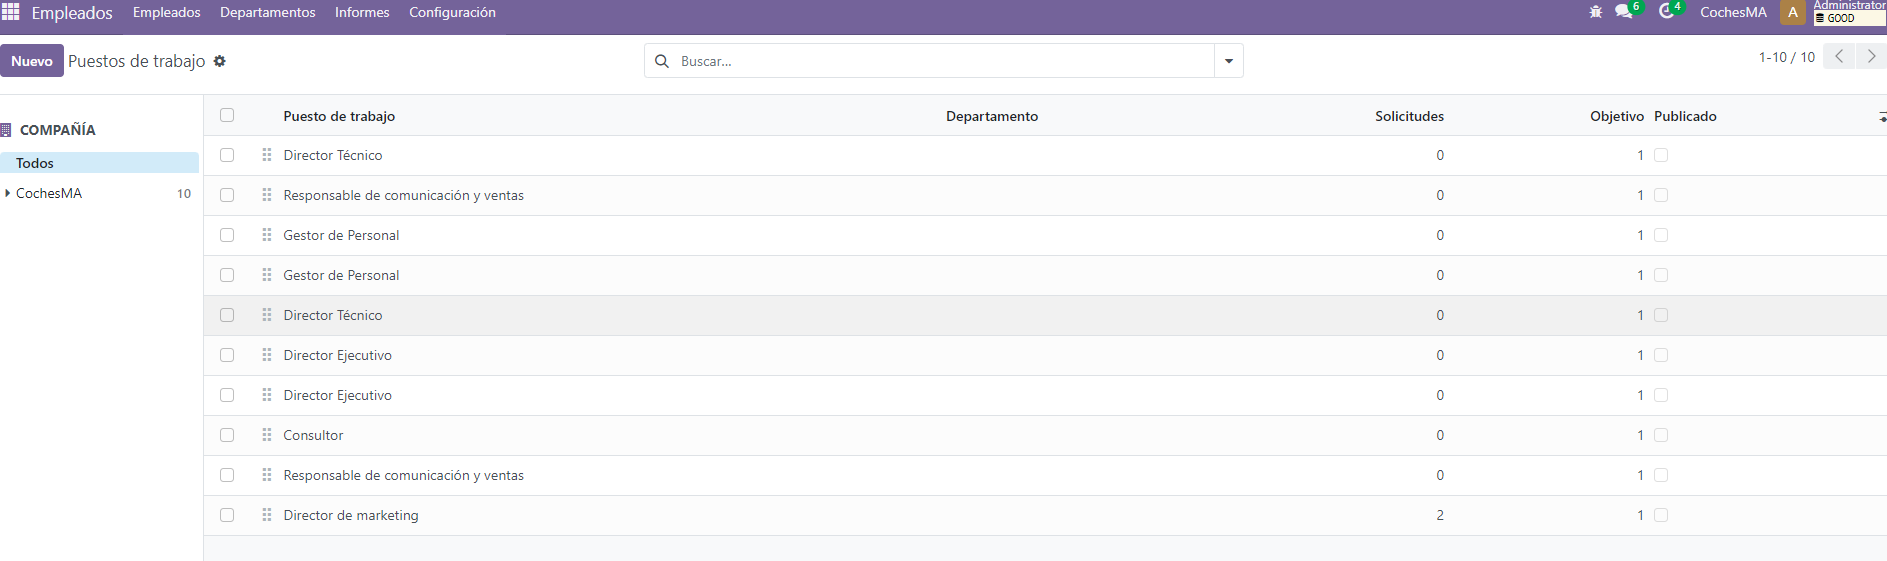
\includegraphics[width=1\linewidth]{fotosGestPers/puestos.png}
    \caption{Lista de departamentos de la compañía}
    \label{fig:enter-label}
\end{figure}
\begin{figure}[h]
    \centering
    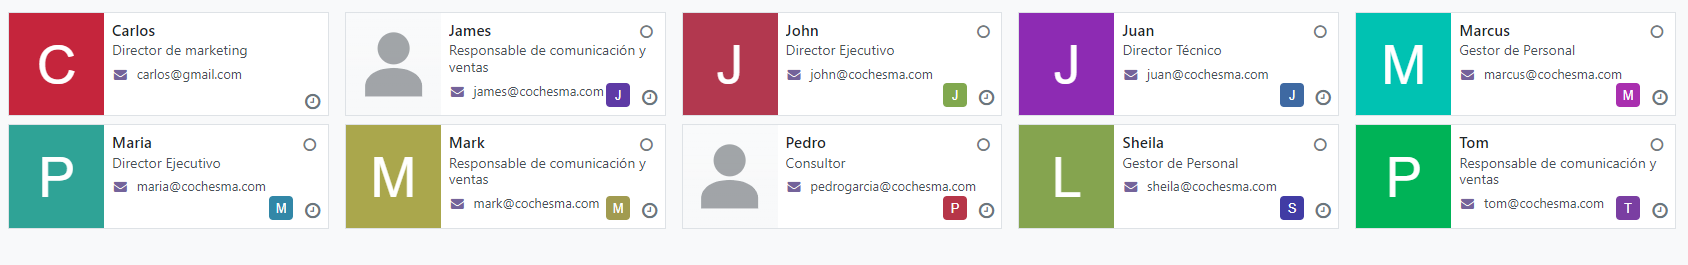
\includegraphics[width=1\linewidth]{fotosGestPers/empleados.png}
    \caption{Lista de empleados de la compañía}
    \label{fig:enter-label}
\end{figure}
\paragraph{}
Se ha creado un nuevo puesto de trabajo, Director de marketing y se ha simulado el proceso de reclutamiento y contratación de un nuevo empleado para este puesto utilizando la vista Kanban de solicitudes.
\begin{figure}[h]
    \centering
    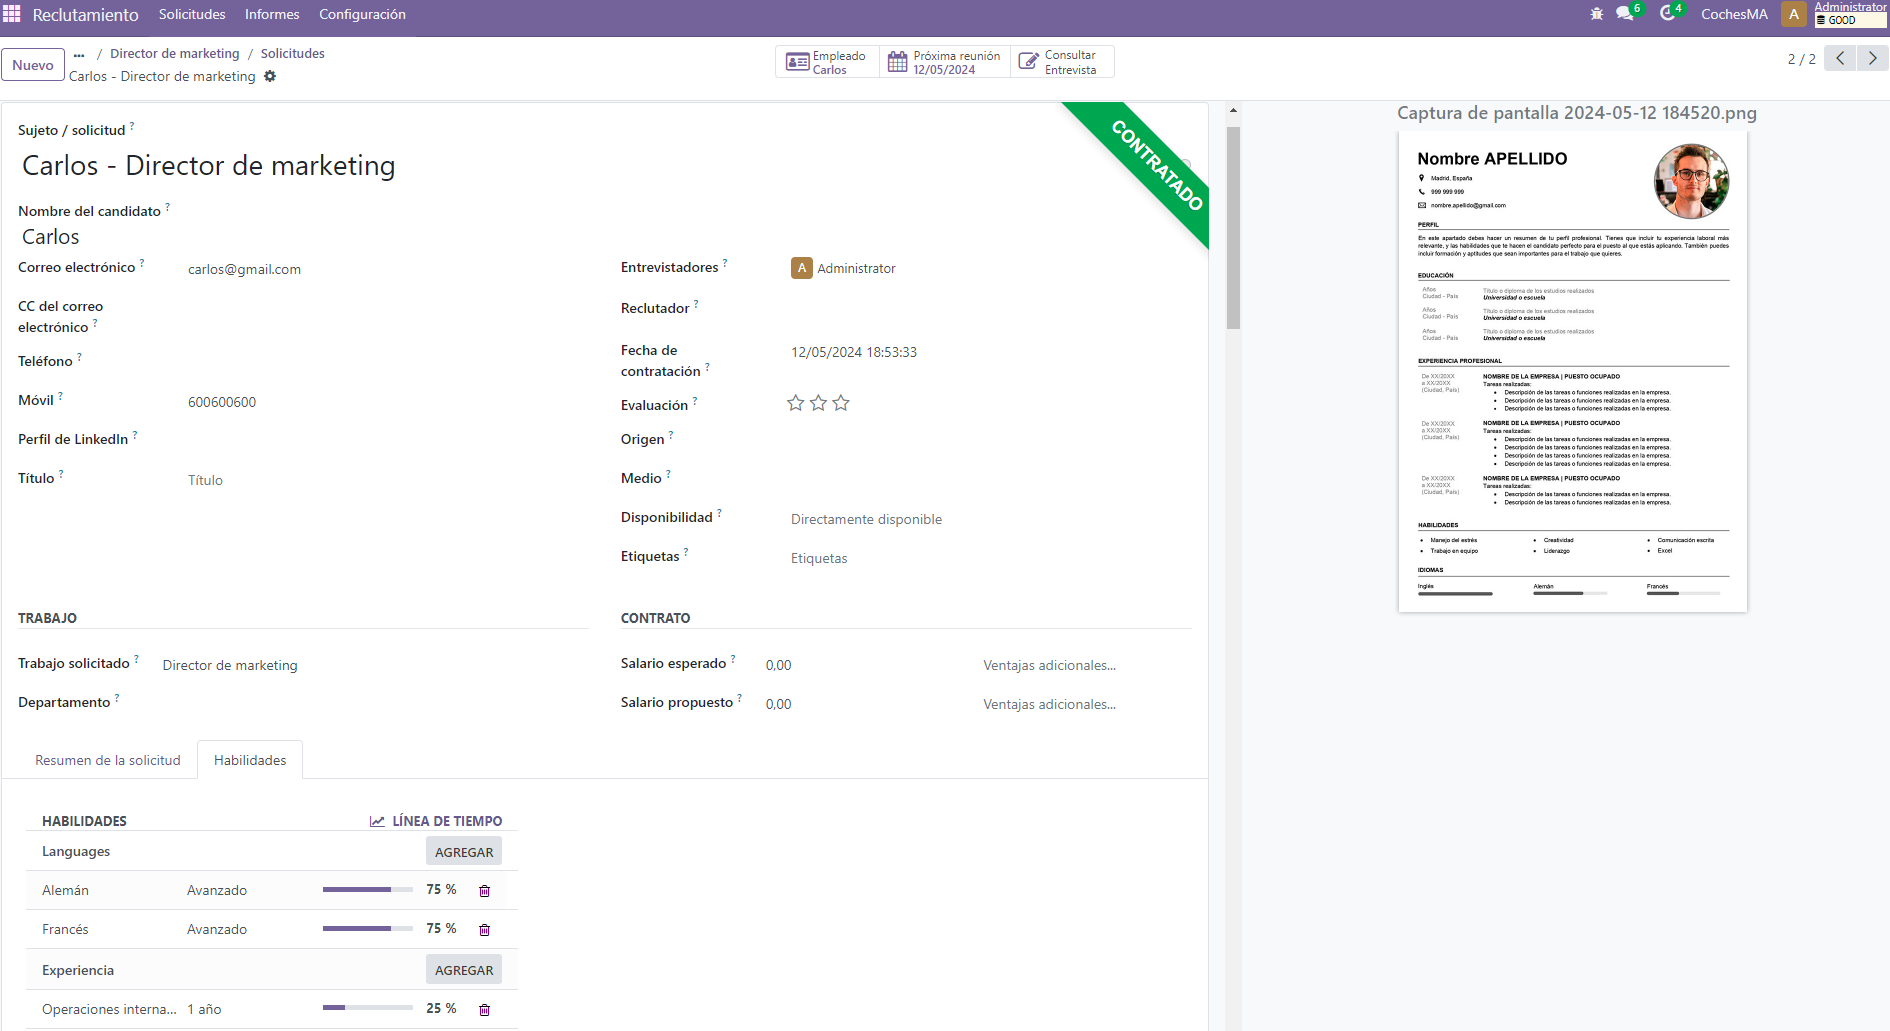
\includegraphics[width=1\linewidth]{fotosGestPers/reclutamiento.png}
    \caption{Solicitud al puesto de Director de marketing}
    \label{fig:enter-label}
\end{figure}
\begin{figure}[h]
    \centering
    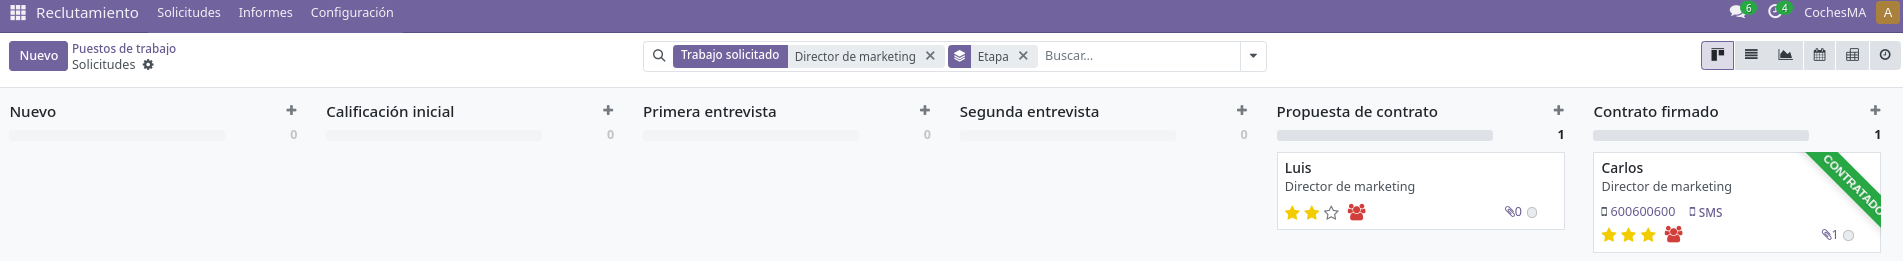
\includegraphics[width=1\linewidth]{fotosGestPers/kanban.png}
    \caption{Vista kanban con los candidatos y su estado e el proceso de reclutamiento}
    \label{fig:enter-label}
\end{figure}
\paragraph{}
Por último, se ha creado un BPMN del proceso de reclutamiento realizado.
\begin{figure}[h]
    \centering
    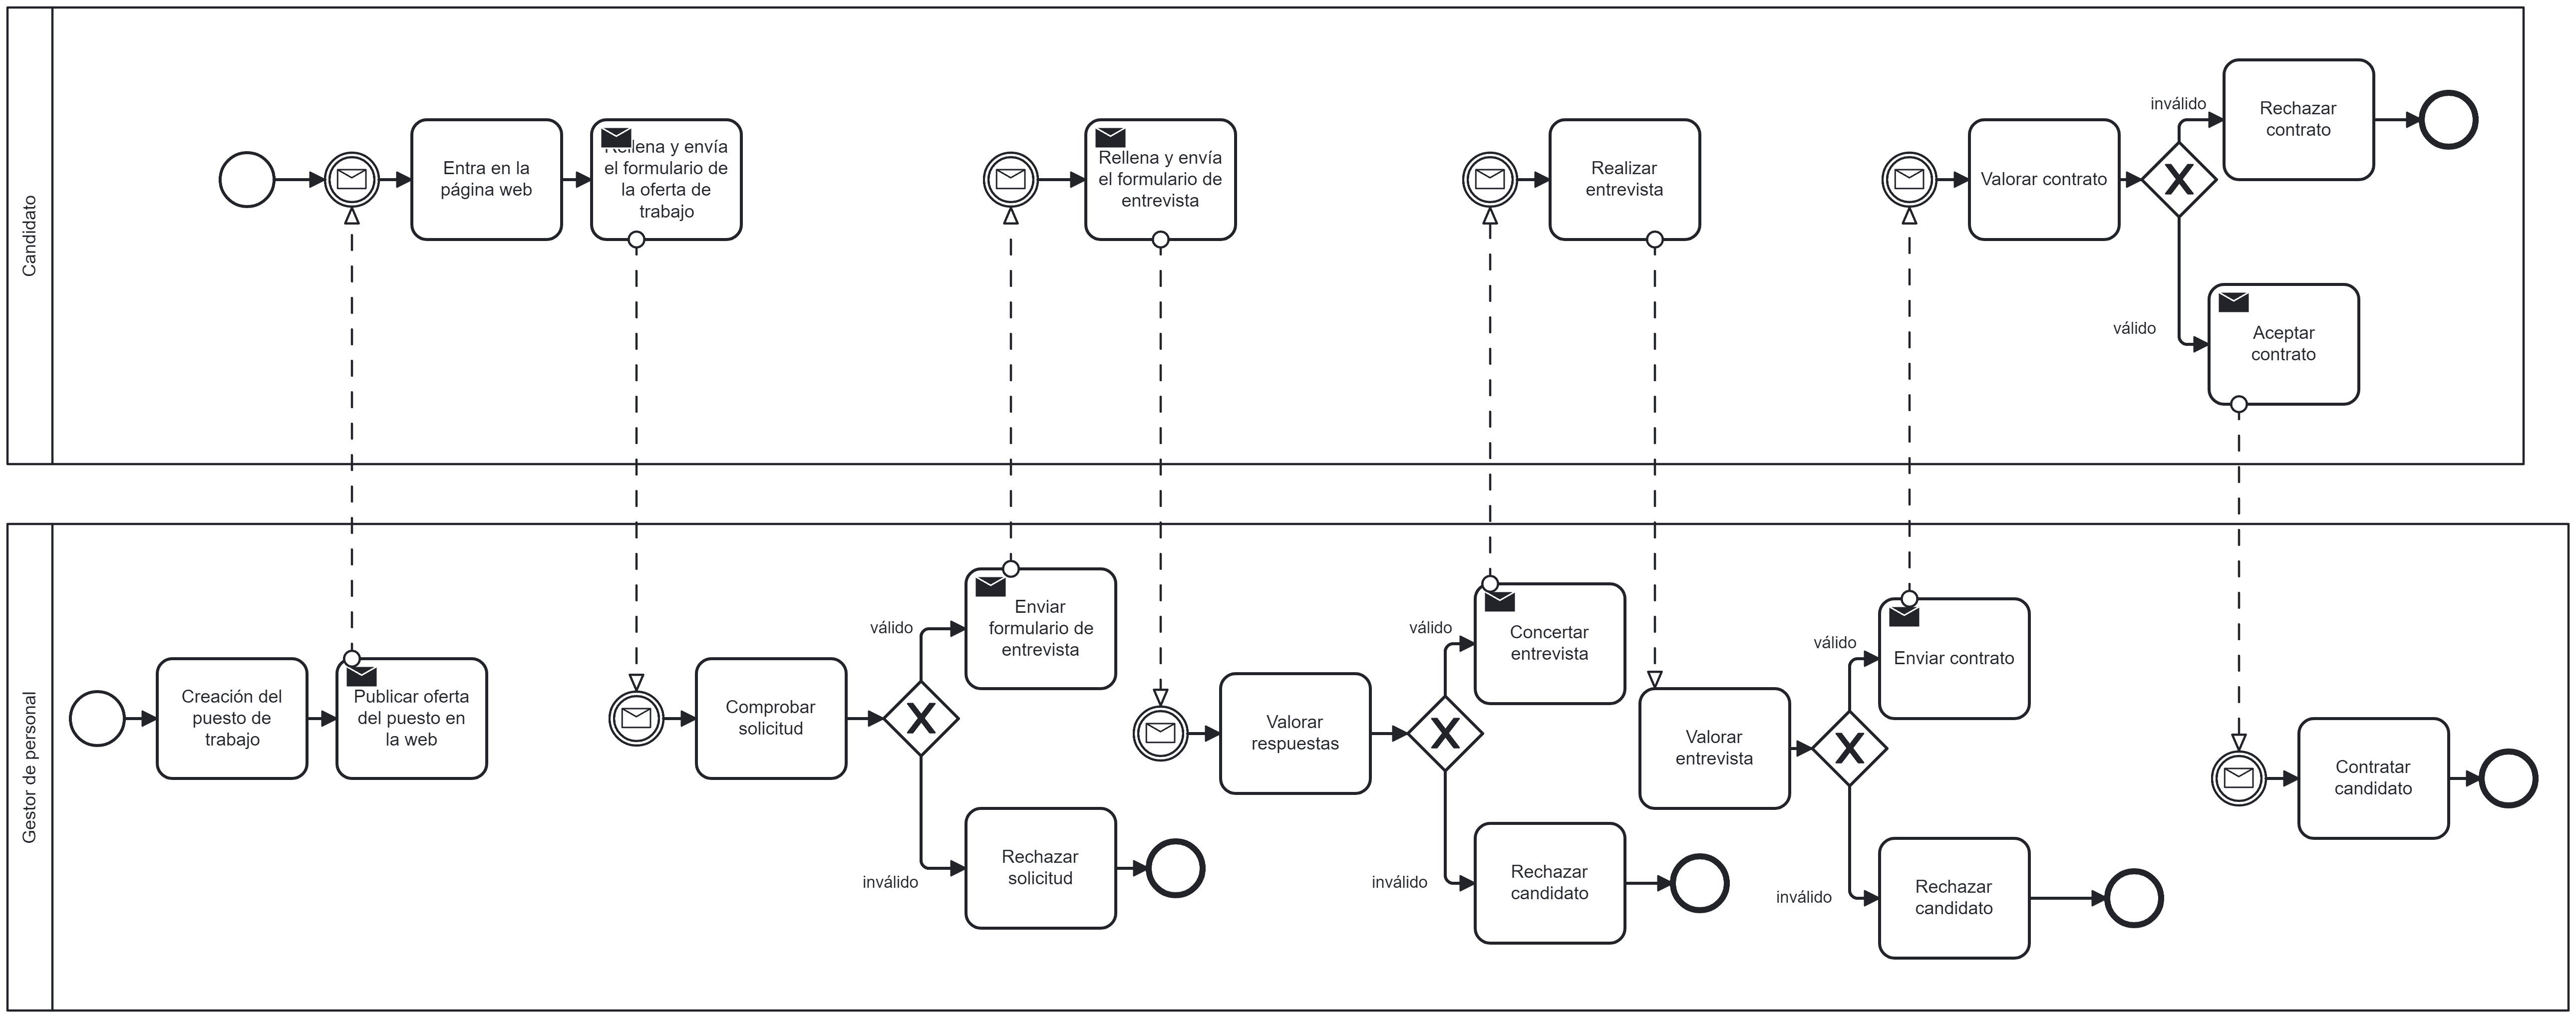
\includegraphics[width=1\linewidth]{bpmn/gestPers.png}
    \caption{Solicitud al puesto de Director de marketing}
    \label{fig:enter-label}
\end{figure}

\subsection{Conclusiones}
\paragraph{}
Durante la evaluación de la gestión de personal en Odoo, hemos observado que la parte relacionada con la creación de departamentos, puestos de trabajo y empleados se llevó a cabo de manera adecuada y eficiente. Se ha demostrado una comprensión clara de cómo configurar la estructura organizativa y asignar roles y responsabilidades dentro de la empresa. 
\paragraph{}
Sin embargo, en lo que respecta al reclutamiento y la gestión de solicitudes, hemos identificado algunos aspectos que requieren mejoras. Por ejemplo, hemos observado la necesidad de añadir manualmente desde Odoo las habilidades, experiencia y lenguaje del candidato, lo cual puede resultar poco práctico al no ser incluido directamente en el proceso de solicitud. Además, es importante tener en cuenta que la eficiencia de la gestión puede disminuir cuando se generan grandes cantidades de empleados.
\paragraph{}
A pesar de ello, es destacable que Odoo ofrece una plataforma sólida para la gestión de personal, con funcionalidades que incluyen diversas formas de evaluar el nivel del candidato, ya sea mediante entrevistas o formularios, lo cual resulta más eficiente.